\documentclass{article}

\usepackage{iclr2027_conference,times}
\usepackage{amsmath,amssymb,amsthm}
\usepackage{array}
\usepackage{booktabs}
\usepackage{etoolbox}
\usepackage{graphicx}
\usepackage{hyperref}
\usepackage{url}
\usepackage{microtype}
\usepackage{float}
\usepackage{placeins}
\hypersetup{hidelinks,hypertexnames=false}
\setlength{\textfloatsep}{7pt plus 1pt minus 2pt}
\setlength{\floatsep}{6pt plus 1pt minus 2pt}
\setlength{\intextsep}{6pt plus 1pt minus 2pt}
\setlength{\abovedisplayskip}{6pt plus 1pt minus 2pt}
\setlength{\belowdisplayskip}{6pt plus 1pt minus 2pt}
\AtBeginEnvironment{table}{\small}
\renewcommand{\arraystretch}{1.02}

\title{Latent State Spectral Transfer:\\Eigenspace Alignment Beyond Eigenvalues}
\author{Anonymous Authors}
\date{}

\newtheorem{theorem}{Theorem}
\newtheorem{proposition}{Proposition}
\newtheorem{lemma}{Lemma}
\newtheorem{corollary}{Corollary}
\DeclareMathOperator{\tr}{tr}
\newcommand{\comm}[2]{[#1,#2]}
\newcommand{\R}{\mathbb{R}}

\begin{document}
\maketitle

\begin{abstract}
% Plan: Establish the spectral-identification problem, state the operator-pair result, summarize the decisive evidence, and derive the methodological consequence.
Spectral analyses of learned dynamics commonly use the eigenvalues of a latent predictor to characterize which modes of a representation are preserved, attenuated, or amplified over time. This interpretation is incomplete, however, because eigenvalues do not specify how an operator is oriented relative to the covariance structure of the latent states on which it acts. We formulate latent transfer as a property of the operator pair $(\Sigma,P)$ together with a declared latent metric $M$. To isolate the missing geometric dependence, we construct an isospectral family $P_\theta=R_\theta\Lambda R_\theta^\top$ whose eigenvalues remain fixed while its eigenspaces rotate relative to those of $\Sigma$. For a rotation restricted to coordinates $(i,j)$, we prove the exact identity $\|[\Sigma,P_\theta]\|_F=|(\sigma_i-\sigma_j)(\lambda_i-\lambda_j)\sin(2\theta)|/\sqrt{2}$. We additionally derive a covariance-basis identity valid for arbitrary, including non-normal, predictors and show how a metric-aware commutator transforms under general invertible latent reparameterizations. Controlled analyses confirm the predicted angular dependence and show that eigenspace rotation at fixed eigenvalues changes covariance-weighted energy transport and the accumulation of multi-step prediction residuals. Gauge and Schur controls distinguish Euclidean coordinate effects from non-normal predictor geometry. We further evaluate the declared diagnostics in representations produced by LeWorldModel, I-JEPA, JEPA-WM, and DINO-WM. Within the declared finite-dimensional operator-pair setting, these findings support a conditional diagnostic conclusion: spectral accounts of latent transfer require either a justified shared basis and metric or explicit covariance--predictor alignment and non-normality measurements. The proposed diagnostic uses no predefined transformation group and is therefore group-unspecified and complementary to equivariant predictive representation learning.
The extension is deliberately stronger than a coordinate change: we prove that
covariance alone cannot define a nontrivial full-GL alignment statistic, and
give a metric-relative Schur--resolvent and local-Jacobian remainder
formulation for non-normal and nonlinear predictors. The resulting object is a
scoped transfer diagnostic, not a universal certificate without a declared
metric, local smoothness bounds, and calibrated prediction error.
\end{abstract}

\section{Introduction}

% Plan: Establish the problem and identify the hidden sufficiency assumption.
Latent predictive models compress observations into representations on which future states, masked regions, or transformed views can be predicted. Their high-dimensional behavior is often summarized spectrally: covariance eigenvalues describe where representation energy is concentrated, while predictor eigenvalues describe the persistence or attenuation of transition modes. Spectral descriptions are central to analyses of frequency bias and operator learning \citep{rahaman2019spectralbias,cao2019spectralbias,tancik2020fourier,hong2022activation,li2021fno,khodakarami2026hfs}. Yet a latent predictor acts on a representation distribution, not in isolation. The scientific question is therefore relational: do its eigenvalues identify which covariance-weighted latent directions are actually transported?

% Plan: Formulate the operator-pair object and the precise identification question.
Eigenvalues determine an operator only up to its eigenbasis and contain no information about its orientation relative to latent covariance. Two predictors can consequently share an identical eigenvalue list while transporting high-variance directions differently. Mapping predictor eigenvalues directly to transfer thus requires an additional condition---a known shared basis, joint diagonalizability, or measured near-commutativity. We formalize this dependence through the pair $(\Sigma_z,P)$, where $\Sigma_z$ is latent covariance and $P$ is a predictive transition or view-induced action. Commutators, principal angles, and spectral-projector overlaps measure the relation between their invariant subspaces. Figure~\ref{fig:intro} illustrates the resulting question in an action-conditioned LeWorldModel transition.

\begin{figure}[H]
  \centering
  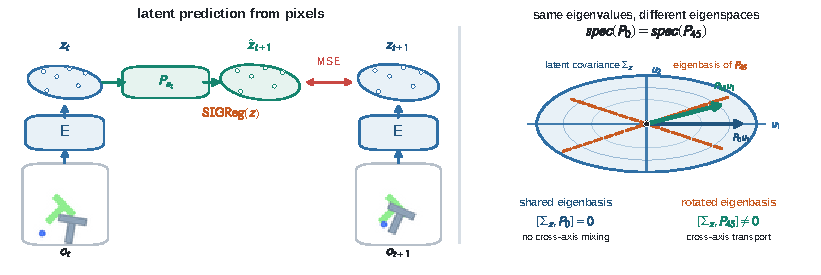
\includegraphics[width=0.97\linewidth]{figures/operator_pair_intro_figure.pdf}
  \caption{One learned-system instance of the operator pair. PushT simulator frames are encoded into adjacent LeWM latents; the action-conditioned predictor produces $\hat z_{t+1}$ under prediction MSE and SIGReg. The resulting latent covariance $\Sigma_z$ and local transition action $P$ instantiate the same operator-pair question studied in the theorem. The same transition spectrum can be aligned or rotated relative to $\Sigma_z$, yielding commuting or noncommuting covariance-relative transport. The geometry is schematic; quantitative changes appear in Figure~\ref{fig:main}.}
  \label{fig:intro}
\end{figure}

% Plan: State the exact theorem and its falsifiable prediction.
Our theoretical result fixes diagonal spectra $\Sigma$ and $\Lambda$ and rotates only the predictor eigenspace, defining $P_\theta=R_\theta\Lambda R_\theta^\top$. Every $P_\theta$ is isospectral, yet we prove that $\|[\Sigma,P_\theta]\|_F$ is proportional to $|(\sigma_i-\sigma_j)(\lambda_i-\lambda_j)\sin(2\theta)|$. The mismatch vanishes at jointly diagonal endpoints, peaks at $45^\circ$, and disappears when either spectrum is flat on the rotated plane. A spectrum-only account predicts invariance across this family; an alignment account predicts the closed-form oblique response and corresponding variation in covariance-weighted transfer. The construction therefore gives both a non-identifiability theorem and a falsifiable signature of the missing geometry.

% Plan: Explain how the controls identify alignment separately from rival factors.
The experiments implement this discriminator. The primary sweep varies only relative eigenspace orientation while holding predictor eigenvalues fixed. Jointly diagonal permutations, spectrum-matched random bases, and flat-spectrum cases test coordinate ordering, arbitrary noncommutativity, and eigengap dependence. Ablations over anisotropy, dimension, filtering, and readout test numerical robustness. The commutator follows the predicted $|\sin(2\theta)|$ law, while covariance-weighted energy transfer and multi-horizon residual growth vary under the same fixed-spectrum perturbation. These controls isolate alignment from spectral shape and metric choice.

% Plan: Establish empirical applicability while preserving the theorem-measurement boundary.
We next evaluate the same quantities in learned representations. Frozen LeWorldModel latents and I-JEPA features exhibit covariance-relative transition and view-displacement structure beyond randomized controls. Released JEPA-WM and DINO-WM checkpoints provide explicit action-conditioned operators, evaluated through cross-fitting, pair-shuffled and spectrum-preserving controls, reconstructed splits, and action-order interventions. The theorem establishes finite-dimensional non-identifiability; these measurements show that alignment, temporal correspondence, prediction error, and action dependence remain empirically separable.

% Plan: State the paper's contributions in conventional scholarly form.
The contributions of this work are fourfold:
\begin{itemize}
  \setlength{\itemsep}{1pt}
  \setlength{\parskip}{0pt}
  \setlength{\parsep}{0pt}
  \item We formulate spectral transfer as an identification problem for $(\Sigma_z,P)$ and prove that predictor eigenvalues alone are insufficient.
  \item We establish a full-$\mathrm{GL}(d)$ identifiability boundary: covariance alone cannot provide a nontrivial gauge-invariant alignment statistic, whereas a declared metric yields a well-defined metric-relative diagnostic.
  \item We extend the certificate beyond symmetric predictors through arbitrary-predictor covariance-basis identities, Schur--resolvent finite-horizon bounds, and a local-Jacobian remainder bound for nonlinear predictors.
  \item We validate the resulting diagnostic protocol in frozen representations and action-conditioned world models using randomized, spectrum-preserving, and held-out controls.
\end{itemize}

% Plan: Conclude with the methodological consequence and exact scope.
The resulting contribution is a conditional certificate protocol with an
explicit scope. A predictor spectrum identifies latent transfer only with a
justified shared-basis condition or an explicit, metric-declared
covariance--predictor alignment statistic; covariance alone cannot define that
statistic under full general-linear gauge freedom. For non-normal predictors,
the report must additionally include Schur-subspace, resolvent, and
non-normality diagnostics, and for nonlinear predictors it must report a
local-Jacobian remainder. This protocol is group-unspecified and complementary
to architectures that impose invariance or equivariance; it is not a claim of
representation-intrinsic validity under arbitrary reparameterization or of a
universal learned-dynamics certificate.

\section{Related Work}

\paragraph{Spectral bias and learned operators.}
Spectral accounts of learning describe mode-dependent approximation, convergence, and generalization. Neural networks often fit low-frequency components before high-frequency components \citep{rahaman2019spectralbias,cao2019spectralbias}, while kernels, Fourier features, architectures, and activations alter the resulting frequency response \citep{jacot2018ntk,tancik2020fourier,hong2022activation,fridovichkeil2022spectralpractice}. The same perspective is central to neural operators: Fourier Neural Operators parameterize mappings in spectral coordinates \citep{li2021fno}, and recent analyses study the loss, recovery, or rescaling of high-frequency content \citep{khodakarami2026hfs,perrone2026freqnodps,xie2026frequencybias,sun2026s2rl}. These works ask how behavior varies across spectral modes. We ask what remains unidentified when those eigenvalues are held fixed.

\paragraph{Latent predictive representations.}
World models learn compact dynamics for prediction, planning, and control \citep{ha2018worldmodels,hafner2020dreamer,hafner2023dreamerv3,micheli2023iris,hansen2024tdmpc2}, whereas image and video JEPAs learn predictive representations without reconstructing pixels \citep{assran2023ijepa,bardes2024vjepa,assran2025vjepa2}. Recent work has extended these ideas to latent planning, temporally extended prediction, stable end-to-end training, and joint-embedding predictive world models \citep{maeslelidec2026lewm,zhang2026hwm,du2026vlwm,ding2026worldmodels,terver2025jepawm}. In all of these systems, a latent covariance describes where representation energy lies and a predictor describes how that representation changes. Our concern is the geometry between those two objects, rather than either spectrum considered separately.

\paragraph{Equivariant predictive world models.}
The closest JEPA precedent to our geometric question is seq-JEPA, which processes short sequences of transformed views, conditions prediction on relative transformations or actions, and uses architectural inductive biases to separate an equivariant view representation from an invariant aggregate representation \citep{ghaemi2025seqjepa}. Its object is transformation-aware representation learning: the architecture specifies, or induces, how a representation should respond to a declared transformation. Our object is an identification question about a learned linear summary: whether a covariance-relative transfer quantity is determined by the predictor eigenvalue list. More explicitly, \emph{seq-JEPA studies how architecture can impose or induce transformation-aware representations; this work studies whether a declared covariance-relative linear transfer quantity is identifiable from predictor eigenvalues}. We therefore do not propose an equivariant architecture, assume a transformation group, or use the commutator as an equivariance certificate. Our diagnostic is \emph{group-unspecified rather than equivariance-aware}: it neither assumes nor tests a particular group representation. The two directions are complementary. Equivariant JEPA can constrain how transformations act, while our metric-aware covariance--predictor measurements test whether the resulting predictor spectrum is sufficient to describe transfer relative to the learned latent geometry.

\paragraph{Representation alignment.}
Representation-alignment work studies whether two learned spaces, or two task-relevant subspaces, encode corresponding directions. Spectral prediction theory separates prediction behavior into contributions from spectral content and alignment with the target \citep{canatar2023spectral}. Latent functional maps instead construct an explicit map between representation spaces and evaluate whether their intrinsic spectral structures correspond \citep{fumero2024lfm}; related cross-modal diagnostics show that similar eigenvalue profiles do not guarantee aligned eigenvector bases \citep{sarkar2026spectralgeometry}. Domain-adaptation methods make a related comparison at the subspace level, where the estimand is the discrepancy between source and target feature subspaces \citep{fernando2014subspace,thopalli2022subspace}. These studies provide the essential distinction between spectral shape and orientation, but their primary object is correspondence between representation spaces (or prediction relative to a target), not the action of a transition operator on a covariance-weighted latent distribution. Our estimand is consequently different: for a fixed latent covariance $\Sigma$ and predictor $P$, we ask whether a declared transfer functional $\mathcal{T}(\Sigma,P)$ is identifiable from the eigenvalues of $P$. The isospectral intervention holds those eigenvalues fixed and changes only the predictor eigenspace, turning alignment from a descriptive similarity score into a falsifiable sufficiency test for spectral transfer.

\paragraph{Simultaneous diagonalization and commuting operators.}
Simultaneous-diagonalization theory asks a structural question: do a collection of operators admit a common basis in which they are all diagonal (or block diagonal), and can that property be estimated from noisy observations? Statistical tests make this question explicit for matrix families \citep{xu2021simdiag}, while matrix analysis characterizes the role of commutation and joint spectral structure \citep{bhatia1997matrix,stewart1990matrix}. For symmetric or, more generally, jointly normal operators, commutation is equivalent to the existence of a common orthogonal/unitary eigenbasis; outside that setting, a small commutator alone does not certify that eigenvectors are well conditioned or that powers of the operator are benign. Work on noncommutative algebras likewise treats failure of commutation as a structural property of the operator family \citep{parada2021noncommutative}. Our use is narrower and more discriminating: simultaneous diagonalization is the \emph{additional condition} under which spectrum-only transfer claims could be justified, whereas the paper tests what happens when that condition is relaxed while the predictor spectrum remains unchanged. Thus the commutator is not proposed as a new diagonalization test; it is one observable in an isospectral identification experiment whose target is covariance-relative transfer.

\paragraph{Non-normal operators and spectral insufficiency.}
For a non-normal predictor, eigenvalues and right-eigenvector angles do not determine the finite-horizon action of the operator. Non-orthogonal eigenvectors, the upper-triangular remainder in a Schur decomposition, pseudospectral sensitivity, and transient amplification can all change $P^h$ without changing the eigenvalue list \citep{bhatia1997matrix,stewart1990matrix,trefethen2005spectra}. This literature therefore provides a second, logically distinct reason that eigenvalue-only summaries can fail: the operator may have non-normal dynamics even after its relation to covariance has been fixed. We separate the two sources rather than fold them into one alignment number. The symmetric isospectral construction isolates covariance--predictor eigenspace rotation; the learned-predictor analysis additionally reports Schur-subspace overlaps and a Schur residual/non-normality index. Consequently, a large covariance commutator is not interpreted as evidence of transient growth, and a non-normality index is not interpreted as evidence of covariance misalignment. The contribution is the joint measurement protocol that keeps these two failure modes identifiable.

\paragraph{Spectral geometry, principal angles, and projectors.}
Spectral geometry supplies basis-robust ways to compare subspaces when individual eigenvectors are ambiguous, repeated, or numerically unstable. Principal-angle algorithms and perturbation bounds quantify the geometry of subspace pairs \citep{bjork1973principal,davis1970rotation,stewart1990matrix}; the $A$-inner-product formulation makes the metric dependence explicit \citep{knyazev2002principal}. Spectral-projector overlaps provide the corresponding invariant quantity for grouped eigenspaces, and functional-map methods use related spectral coordinates to compare representations \citep{fumero2024lfm,sarkar2026spectralgeometry}. We use these tools for a different purpose: not to declare two representations aligned in the abstract, but to measure the relation between covariance eigenspaces and predictor invariant subspaces under a declared latent metric, and then test whether that relation changes a transfer readout at fixed predictor spectrum. The distinction matters because a projector overlap is a geometric descriptor, whereas identifiability asks whether all operators sharing the reported spectrum have the same value of the downstream quantity.

\paragraph{Positioning of this work.}
Across these literatures, representation alignment measures correspondence between spaces, simultaneous diagonalization tests whether a shared basis exists, non-normal analysis explains why eigenvalues can miss finite-horizon behavior, and spectral geometry supplies invariant subspace measurements. None of these objects, by itself, answers the fixed-spectrum question posed here: can a declared covariance-relative linear transfer quantity be recovered from predictor eigenvalues alone? We answer it by constructing an isospectral family, rotating the predictor eigenspace relative to covariance, and jointly reporting the metric-aware commutator, principal angles, projector overlaps, and non-normality controls. The resulting contribution is therefore not a generic alignment score or an equivariance criterion; it is a falsifiable diagnostic of when a spectrum-only explanation is, and is not, identified.

\section{Method}

\paragraph{Finite-dimensional transfer model.}
We study finite-dimensional latent transfer through a covariance operator $\Sigma\in\R^{d\times d}$ and a predictor operator $P\in\R^{d\times d}$. The covariance assigns energy to latent directions, while the predictor transports that energy through a one-step transition. The spectrum of $P$ identifies transfer only if all predictors with that spectrum induce the same covariance-relative transfer functional.

\paragraph{Latent metric and coordinate gauge.}
The ordinary Euclidean commutator implicitly fixes a metric on latent
coordinates. To make this choice explicit, let $M\succ0$ denote the declared
latent metric and represent the covariance as a contravariant matrix. The
corresponding covariance endomorphism is $S_M=\Sigma M$, and we define
\begin{equation}
\label{eq:metric-aware-commutator}
\mathcal{C}_M(\Sigma,P)=
\frac{\|[S_M,P]\|_M}{\|S_M\|_M\|P\|_M},\qquad
\|K\|_M^2=\tr(K^\top M K M^{-1}).
\end{equation}
Under a general invertible reparameterization $z'=Az$, the objects transform
as $\Sigma'=A\Sigma A^\top$, $P'=APA^{-1}$, and
$M'=A^{-\top}MA^{-1}$. Hence $S_M'=AS_MA^{-1}$ and
$\mathcal{C}_{M'}(\Sigma',P')=\mathcal{C}_M(\Sigma,P)$. The ordinary
Euclidean statistic is recovered with $M=I$; it is invariant under orthogonal
changes of coordinates but not under arbitrary rescaling or whitening. All
learned-system measurements therefore report the latent metric (or explicitly
label the result as Euclidean-gauge dependent).

\paragraph{Gauge identifiability boundary.}
The metric is not a cosmetic normalization. Under the full group of invertible
latent reparameterizations, covariance alone cannot support a nontrivial
covariance--predictor eigenspace alignment statistic. Choosing the
covariance-induced metric $M=\Sigma^{-1}$ gives
\begin{equation}
\bar S_M=M^{1/2}\Sigma M^{1/2}=I,
\qquad
\bar P_M=M^{1/2}PM^{-1/2},
\label{eq:covariance-only-gauge-collapse}
\end{equation}
so $[\bar S_M,\bar P_M]=0$ for every predictor. A nonzero alignment
measurement under the full-GL gauge therefore requires additional structure,
such as a decoder pullback metric, an observation-space metric, or an
action/goal metric. In declared metric coordinates,
\begin{equation}
\bar S_M=M^{1/2}\Sigma M^{1/2},
\qquad
\bar P_M=M^{1/2}PM^{-1/2},
\label{eq:metric-whitened-pair}
\end{equation}
the pair is unique up to orthogonal similarity. Projector overlaps, Schur
subspaces, and Frobenius diagnostics are then gauge-invariant relative to the
declared metric, while the Euclidean special case remains explicitly
gauge-dependent.

\paragraph{Same-spectrum construction.}
Let
\begin{equation}
\label{eq:isospectral-diagonals}
\begin{aligned}
\Sigma=\mathrm{diag}(\sigma_1,\ldots,\sigma_d),\qquad
\Lambda=\mathrm{diag}(\lambda_1,\ldots,\lambda_d).
\end{aligned}
\end{equation}
For coordinates $i\neq j$, let $R_\theta$ be the identity outside the $(i,j)$ plane and a two-dimensional rotation inside that plane. The same-spectrum predictor family is
\begin{equation}
P_\theta=R_\theta\Lambda R_\theta^\top .
\label{eq:isospectral-family}
\end{equation}
All members of the family in Eq.~\eqref{eq:isospectral-family} have spectrum $\{\lambda_1,\ldots,\lambda_d\}$. The construction therefore changes predictor eigenspaces while holding predictor eigenvalues fixed. Any quantity that changes with $\theta$ is not determined by the predictor spectrum alone.

\paragraph{Eigenspace-alignment measurements.}
We measure covariance-predictor eigenspace mismatch by
\begin{equation}
\mathcal{C}(\theta)=
\frac{\|\comm{\Sigma}{P_\theta}\|_F}
{\|\Sigma\|_F\|P_\theta\|_F}.
\label{eq:normalized-commutator}
\end{equation}
The normalized commutator in Eq.~\eqref{eq:normalized-commutator} vanishes when the two operators commute and increases with their covariance-relative eigenspace mismatch.

The same relation can be described through spectral projectors. If $\Pi_a^\Sigma$ and $\Pi_b^P$ denote covariance and predictor eigenspace projectors, then
\begin{equation}
\mathcal{O}_{ab}=\|\Pi_a^\Sigma\Pi_b^P\|_F^2
\label{eq:projector-overlap}
\end{equation}
records eigenspace overlap, equivalently the squared cosines of principal angles for simple subspaces. We use Eq.~\eqref{eq:normalized-commutator} in the main theorem because it admits a closed-form curve; Eq.~\eqref{eq:projector-overlap} provides the corresponding subspace-level vocabulary for learned representations.

For non-normal predictors, right eigenvectors need not be orthogonal and can be
ill-conditioned. We therefore complement projector measurements with the
Schur-based non-normality index
\begin{equation}
\label{eq:nonnormality-index}
\nu(P)=\frac{\|P^\top P-PP^\top\|_F}{\|P\|_F^2},
\end{equation}
and treat covariance--Schur-subspace overlap as the primary subspace statistic.
For a nonlinear predictor $f$, $P$ denotes a declared local Jacobian or
cross-fitted linearization $J_f(z,a)$, and all reported quantities are indexed
by state, action condition, and horizon rather than interpreted as one global
operator.

\paragraph{Transfer readouts.}
We use two transfer readouts. For a top coordinate band $B_k$, the top-band lift compares predicted energy in $B_k$ to the isotropic baseline,
\begin{equation}
\mathcal{T}_{k,h}(P_\theta)=
\frac{\tr(\Pi_k P_\theta^h\Sigma (P_\theta^h)^\top)}
{\tr(P_\theta^h\Sigma (P_\theta^h)^\top)}
\bigg/ \frac{k}{d},
\label{eq:top-band}
\end{equation}
where $\Pi_k$ projects onto the first $k$ coordinates. Residual growth compares residual trace at a long horizon to residual trace at the first horizon under the same synthetic generator. These deterministic readouts quantify covariance-relative transfer across horizons.

The diagonal-transfer generator used by the analytical sweeps gives this residual readout a concrete form. Let $\rho_j$ be the coordinate-$j$ predictor response and let $\tilde\sigma_j$ be the heat-filtered latent variance. At horizon $h$, the predicted trace and residual trace are
\begin{subequations}
\label{eq:trace-readouts}
\begin{align}
\mathcal{P}_h&=\sum_{j=1}^d \tilde\sigma_j\rho_j^h,
\label{eq:predicted-trace}\\
\mathcal{E}_h&=\sum_{j=1}^d \tilde\sigma_j(1-\rho_j^h)^2 .
\label{eq:residual-growth}
\end{align}
\end{subequations}
We summarize multi-horizon accumulation in Eq.~\eqref{eq:residual-growth} by $\mathcal{E}_8/\mathcal{E}_1$, the ratio of long-horizon to one-step residual trace.

\section{Theoretical Analysis}

\begin{theorem}[Single-Plane Same-Spectrum Commutator Identity]
\label{thm:single-plane}
Let $\Sigma$ and $\Lambda$ be diagonal. Let $P_\theta=R_\theta\Lambda R_\theta^\top$, where $R_\theta$ rotates only coordinates $(i,j)$. Then
\begin{equation}
\|\comm{\Sigma}{P_\theta}\|_F
=
\frac{|(\sigma_i-\sigma_j)(\lambda_i-\lambda_j)\sin(2\theta)|}{\sqrt{2}} .
\label{eq:single-plane-identity}
\end{equation}
After normalization by $\|\Sigma\|_F\|P_\theta\|_F$, the same $|\sin(2\theta)|$ dependence remains. The curve is zero at $\theta=0^\circ$ and $\theta=90^\circ$, maximized at $\theta=45^\circ$, and identically zero if either spectrum is flat on the rotated plane.
\end{theorem}

Theorem~\ref{thm:single-plane}, through the identity in Eq.~\eqref{eq:single-plane-identity}, gives a direct identification result. The eigenvalues of $P_\theta$ are invariant in $\theta$, so any statistic that changes with $\theta$ cannot be determined by the predictor spectrum alone. The commutator is the lowest-order witness that the covariance and predictor are not jointly diagonal in the same basis.

\begin{proposition}[Covariance-basis identity for arbitrary predictors]
\label{prop:arbitrary-predictor-commutator}
Let $\Sigma=U\operatorname{diag}(\sigma_1,\ldots,\sigma_d)U^\top$
be symmetric positive semidefinite and let $P\in\R^{d\times d}$ be arbitrary,
without a symmetry or normality assumption. Writing
$\widetilde P=U^\top P U$, we have
\begin{equation}
\label{eq:arbitrary-predictor-identity}
\|[\Sigma,P]\|_F^2
=\sum_{r,s=1}^d(\sigma_r-\sigma_s)^2
\left|\widetilde P_{rs}\right|^2.
\end{equation}
Thus the commutator measures covariance-weighted off-diagonal coupling in
the covariance eigenbasis for arbitrary predictors; it is not an eigenvector
angle certificate for non-normal predictors.
\end{proposition}

\paragraph{Proof.}
Orthogonal invariance gives
$\|[\Sigma,P]\|_F=\|[\operatorname{diag}(\sigma),\widetilde P]\|_F$.
The $(r,s)$ entry of the latter commutator is
$(\sigma_r-\sigma_s)\widetilde P_{rs}$, and summing its squared magnitudes
proves Eq.~\eqref{eq:arbitrary-predictor-identity}. For a non-normal $P$,
Eq.~\eqref{eq:arbitrary-predictor-identity} remains valid, but the eigenvalue
list and right-eigenspace angles do not characterize the transient action of
$P$. We therefore report $\nu(P)$ and Schur-subspace overlaps alongside the
commutator in learned predictors.

\paragraph{Proof sketch.}
Only the rotated two-dimensional block contributes to the commutator. Write $c=\cos\theta$, $s=\sin\theta$, $\Delta_\sigma=\sigma_i-\sigma_j$, and $\Delta_\lambda=\lambda_i-\lambda_j$. In the rotated plane,
\begin{equation}
P_{\theta,ij}=
\begin{bmatrix}
\lambda_i c^2+\lambda_j s^2 & \Delta_\lambda cs\\
\Delta_\lambda cs & \lambda_i s^2+\lambda_j c^2
\end{bmatrix},
\label{eq:rotated-block}
\end{equation}
while $\Sigma_{ij}$ remains diagonal. Substituting Eq.~\eqref{eq:rotated-block} into the commutator gives
\begin{equation}
\comm{\Sigma}{P_\theta}_{ij}=
\begin{bmatrix}
0 & \Delta_\sigma\Delta_\lambda cs\\
-\Delta_\sigma\Delta_\lambda cs & 0
\end{bmatrix}.
\label{eq:commutator-block}
\end{equation}
Taking the Frobenius norm of Eq.~\eqref{eq:commutator-block} gives $2(\Delta_\sigma\Delta_\lambda cs)^2=(\Delta_\sigma\Delta_\lambda)^2\sin^2(2\theta)/2$. All other blocks vanish, and orthogonal conjugation keeps $\|P_\theta\|_F=\|\Lambda\|_F$, so normalization does not change the angular dependence.

\begin{theorem}[Metric-relative Schur transfer bound]
\label{thm:metric-schur-transfer}
Let $M\succ0$, let $P\in\R^{d\times d}$ be arbitrary, and let
$\bar P_M=M^{1/2}PM^{-1/2}=Q T Q^\top$ be a real Schur decomposition with
$T=D+N$, where $D$ is block diagonal and $N$ is strictly block upper
triangular. Define
\begin{equation}
G_{h,M}(P)=\|\bar P_M^h\|_2,
\qquad
\nu_M(P)=
\frac{\|\bar P_M^\top\bar P_M-\bar P_M\bar P_M^\top\|_F}
{\|\bar P_M\|_F^2}.
\label{eq:metric-schur-quantities}
\end{equation}
Then $G_{h,M}$, $\nu_M$, and Schur-subspace projector overlaps are invariant
under $z'=Az$ when $M'=A^{-\top}MA^{-1}$ and $P'=APA^{-1}$. Moreover, for
any contour $\Gamma$ enclosing the spectrum of $\bar P_M$,
\begin{equation}
G_{h,M}(P)
\leq \frac{1}{2\pi}\oint_\Gamma
|\zeta|^h\|(\zeta I-\bar P_M)^{-1}\|_2\,|d\zeta| .
\label{eq:schur-resolvent-bound}
\end{equation}
Consequently, the eigenvalue multiset alone cannot determine finite-horizon
transfer whenever the Schur remainder $N$ or the resolvent norm varies within
an isospectral family.
\end{theorem}

\begin{proof}
Let $U=M'^{1/2}AM^{-1/2}$. From
$M'=A^{-\top}MA^{-1}$, $U$ is orthogonal, and hence
$\bar P_{M'}'=U\bar P_MU^\top$. Orthogonal similarity preserves powers,
the Frobenius departure from normality, and the Frobenius overlaps of
orthogonally transformed projectors. The resolvent inequality follows from
the Dunford--Cauchy representation
$\bar P_M^h=(2\pi i)^{-1}\oint_\Gamma
\zeta^h(\zeta I-\bar P_M)^{-1}d\zeta$ and the triangle inequality.
The final statement follows by taking $T_\alpha=D+\alpha N$ with fixed
diagonal blocks: its eigenvalue multiset is constant, while $T_\alpha^h$
and its resolvent generally vary with $\alpha$.
\end{proof}

\begin{proposition}[Alignment and transient amplification are distinct]
\label{prop:alignment-transient-separation}
Let $\bar S_M\succeq0$ and let $\bar P_M$ be arbitrary. Define the
covariance-weighted finite-horizon energy and operator gain by
\begin{equation}
\label{eq:covariance-weighted-gain}
\mathcal E_{h,M}(P)=\tr\!\left(\bar P_M^h\bar S_M
 (\bar P_M^h)^\top\right),
\qquad G_{h,M}(P)=\|\bar P_M^h\|_2.
\end{equation}
Then
\begin{equation}
\label{eq:covariance-energy-gain-bound}
\mathcal E_{h,M}(P)\leq G_{h,M}(P)^2\tr(\bar S_M).
\end{equation}
The metric-relative commutator measures covariance-basis coupling, whereas
$G_{h,M}$ measures finite-horizon amplification. Neither quantity determines
the other without additional assumptions. In particular, for
$\bar S_M=I$ and
\begin{equation}
\label{eq:fixed-spectrum-jordan-counterexample}
\bar P_\kappa=
\begin{bmatrix}r&\kappa\\0&r\end{bmatrix},\qquad 0<r<1,
\end{equation}
the commutator is zero and the eigenvalue multiset is fixed, but
\begin{equation}
\label{eq:jordan-power-counterexample}
\bar P_\kappa^h=
\begin{bmatrix}r^h&h\kappa r^{h-1}\\0&r^h\end{bmatrix}
\end{equation}
varies with $\kappa$ and can exhibit transient amplification.
\end{proposition}

\begin{proof}
For positive semidefinite $\bar S_M$,
$\tr(A\bar S_MA^\top)\leq\|A\|_2^2\tr(\bar S_M)$; setting
$A=\bar P_M^h$ proves Eq.~\eqref{eq:covariance-energy-gain-bound}.
The covariance-basis identity shows that the commutator depends on weighted
off-diagonal entries of $\bar P_M$, while the Jordan family has
$[I,\bar P_\kappa]=0$ for every $\kappa$. Direct multiplication gives
Eq.~\eqref{eq:jordan-power-counterexample}, proving that zero alignment
commutator and fixed eigenvalues do not rule out transient amplification.
\end{proof}

This proposition supplies the missing interpretation of the Schur extension.
In $\bar P_M=Q(D+N)Q^\top$, $D$ carries the eigenvalue blocks, $N$ carries
upper-triangular non-normal coupling, and the resolvent
$\|(\zeta I-\bar P_M)^{-1}\|$ controls how that coupling is amplified over a
finite horizon. The commutator is therefore neither a proxy for $N$ nor a
proxy for $G_{h,M}$: a complete non-normal report must include all three
layers, together with the covariance-weighted readout in
Eq.~\eqref{eq:covariance-weighted-gain}.

\begin{proposition}[Local nonlinear transfer remainder]
\label{prop:nonlinear-jacobian-remainder}
Let $f_t$ be $C^2$ maps on a tube containing two trajectories, let
$z_{t+1}=f_t(z_t)$, and write $J_t=Df_t(z_t)$. Suppose that, in the
$M$-norm, $\|Df_t(x)\|_M\leq m_t$ and
$\|Df_t(x)-Df_t(y)\|_M\leq H_t\|x-y\|_M$ throughout the tube. For an
initial perturbation $\delta$, define the nonlinear displacement
$u_h=f_{h-1}\circ\cdots\circ f_0(z_0+\delta)-z_h$ and the local linear
prediction $\Phi_h\delta$ with $\Phi_h=J_{h-1}\cdots J_0$. Then
\begin{equation}
\|u_h-\Phi_h\delta\|_M
\leq \frac{\|\delta\|_M^2}{2}
\sum_{j=0}^{h-1}H_j
\left(\prod_{r=0}^{j-1}m_r\right)^2
\left(\prod_{r=j+1}^{h-1}m_r\right).
\label{eq:nonlinear-jacobian-remainder}
\end{equation}
Thus a nonlinear transfer diagnostic must report local Jacobians together
with a Jacobian-Lipschitz/remainder estimate; a global predictor spectrum is
not a certificate for nonlinear multi-step transfer.
\end{proposition}

\begin{proof}
Let $v_t$ be the nonlinear displacement and $e_t=v_t-\Phi_t\delta$.
Taylor's theorem gives
$\|f_t(z_t+v_t)-f_t(z_t)-J_tv_t\|_M\leq H_t\|v_t\|_M^2/2$.
The tube Lipschitz condition gives
$\|v_t\|_M\leq(\prod_{r=0}^{t-1}m_r)\|\delta\|_M$,
while $e_{t+1}=J_te_t+r_t$. Unrolling this recursion yields
Eq.~\eqref{eq:nonlinear-jacobian-remainder}.
\end{proof}

\begin{proposition}[Same-Spectrum Ambiguity]
\label{prop:under-id}
Assume $(\sigma_i-\sigma_j)(\lambda_i-\lambda_j)\neq 0$. The family $\{P_\theta:\theta\in[0,\pi/2]\}$ has a constant predictor spectrum but a nonconstant alignment statistic $\mathcal{C}(\theta)$. Therefore the predictor eigenvalue list alone cannot identify commutator-sensitive covariance-predictor alignment for the pair $(\Sigma,P_\theta)$.
\end{proposition}

\begin{proposition}[Fixed-Spectrum Transfer Readout Variation]
\label{prop:transfer-varies}
In the same two-dimensional rotated plane, let $\Pi_i$ project onto coordinate $i$. Define the horizon-one coordinate energy and its closed form by
\begin{subequations}
\label{eq:coordinate-energy}
\begin{equation}
Q_i(\theta)=\tr(\Pi_i P_\theta\Sigma P_\theta^\top).
\label{eq:coordinate-energy-definition}
\end{equation}
\begin{equation}
\begin{aligned}
Q_i(\theta)
&=
\sigma_i(\lambda_i\cos^2\theta+\lambda_j\sin^2\theta)^2\\
&\quad+
\sigma_j(\lambda_i-\lambda_j)^2\cos^2\theta\sin^2\theta .
\end{aligned}
\label{eq:coordinate-energy-expansion}
\end{equation}
\end{subequations}
Thus the coordinate-energy readout in Eq.~\eqref{eq:coordinate-energy-expansion} varies with $\theta$ while the predictor eigenvalues remain fixed.
\end{proposition}

The identity also specifies when the effect disappears. If the latent covariance or predictor spectrum is flat on the rotated plane, the commutator is zero for every angle. A coordinate permutation of a jointly diagonal pair likewise preserves commutativity. A random basis can create a nonzero commutator, but need not reproduce the structured oblique peak of a single-plane rotation. These cases motivate the controls below.

\begin{corollary}[What Spectra Can and Cannot Certify]
Spectrum shape controls the scale of the alignment effect through the eigengaps $(\sigma_i-\sigma_j)$ and $(\lambda_i-\lambda_j)$, but the predictor spectrum alone cannot certify the effect. A complete spectral-transfer analysis must specify at least one pairwise relation between the latent geometry and transition operator, such as a commutator norm or eigenspace-overlap statistic.
\end{corollary}

Eigenvalue decay describes how mass is distributed over predictor modes; eigenspace alignment determines whether those modes coincide with the covariance directions whose transfer is being interpreted. The two quantities answer different questions and must be reported accordingly.

\section{Experiments}

The analytical experiments are deterministic, allowing the spectrum-only explanation to be tested without estimation noise. We use $d=64$, power-law latent and predictor spectra, rotation angles $\{0,15,30,45,60,75,90\}$ degrees, horizons $\{1,2,4,8\}$, and top bands $k\in\{4,8,16,32\}$. The rotated plane is formed by the first and last coordinates, with latent and predictor eigengaps $0.984375$ and $0.875$. Within each sweep, the quantities not under study are fixed by construction.

The comparison design separates basis alignment from spectral shape. The angle sweep varies only the predictor basis; the permutation-preserving and random-basis controls retain the predictor spectrum while changing the way it is positioned; and the factor-isolating ablations hold either the spectrum or the alignment angle fixed. Additional readouts, dimensions, and nuisance perturbations are reported in the supplement.

The learned-representation experiments instantiate the operator-pair question at two levels. First, frozen LeWorldModel PushT latents and frozen I-JEPA image features test covariance-relative displacement measurements without fitting a temporal operator. The PushT analysis compares dynamics, planner-weighted dynamics, prediction residuals, and transition overlap with norm-matched controls, label shuffles, and a random-subspace null. The I-JEPA analysis measures whether deterministic view displacements concentrate in the covariance eigenspace of source features across six vision benchmarks.

Second, released JEPA-WM and DINO-WM checkpoints test explicit action-conditioned operator estimates. The four checkpoint--environment combinations comprise JEPA-WM and DINO-WM on PushT and PointMaze at horizons $h\in\{1,2,4\}$. Full-rank commutators are paired with cross-fitted low-rank operators, pair-shuffled and spectrum-preserving controls, within-episode action-order derangements, and alternative PointMaze memberships. Together these comparisons separate prediction error, temporal correspondence, and covariance--operator alignment.

\section{Results and Analysis}

We first test identifiability with the isospectral construction, then isolate
eigenspace alignment with controlled perturbations, and finally examine how the
same measurements behave in frozen representations and held-out temporal
operators. This sequence moves from an exact algebraic statement to its
empirical measurement consequences.

\begin{figure}[t]
  \centering
  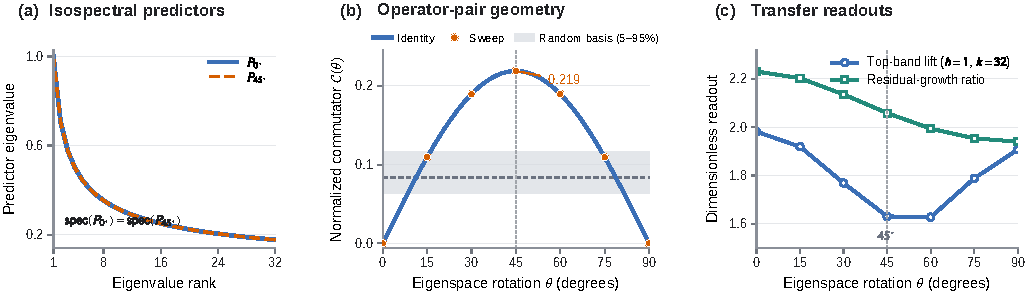
\includegraphics[width=\linewidth]{figures/operator_pair_main_figure.pdf}
  \caption{Same eigenvalues do not imply the same transfer. The left panel shows that the aligned predictor $P_{0^\circ}$ and oblique predictor $P_{45^\circ}$ have the same eigenvalue list. The center panel rotates only the predictor eigenspace relative to the covariance eigenspace, raising the normalized commutator from $0.000$ to $0.219$ and tracing the exact $|\sin(2\theta)|$ witness above the spectrum-matched random-basis null. The right panel shows the resulting changes in top-band lift and residual growth, motivating alignment statistics alongside eigenvalue reports.}
  \label{fig:main}
\end{figure}

Figure~\ref{fig:main} exhibits the identification failure under a fixed spectrum. The commutator rises from zero at $0^\circ$ to $0.219063$ at $45^\circ$ and returns to numerical zero at $90^\circ$, although the predictor eigenvalues never change. The structured peak also exceeds the random-basis reference, whose mean is $0.0836631$ and whose 5th--95th percentile interval is $[0.0637529,0.11723]$. Transfer changes with the same rotation: for top-$k=32$, horizon-1 top-band lift falls from $1.98127$ at alignment to $1.63077$ at $45^\circ$, while residual-growth ratio changes from $2.23004$ to $2.05798$. Predictors that are indistinguishable by eigenvalues are therefore distinguishable by covariance-relative transfer.

The full rotation table in the supplement follows the theorem's exact symmetric curve across all tested angles: $0.000000$, $0.109531$, $0.189714$, $0.219063$, $0.189714$, $0.109531$, and $0.000000$ from $0^\circ$ to $90^\circ$. The projector-based transfer readouts additionally inherit the ordered covariance coordinates, so they distinguish rotations on opposite sides of $45^\circ$ even when the commutator magnitudes agree. This difference links the basis-invariant mismatch witness to the coordinate-specific transfer quantity of interest.

\begin{table}[t]
\centering
\caption{Spectrum-preserving basis perturbations. All rows keep the same predictor eigenvalues. Larger $\mathcal C$ indicates greater covariance--predictor eigenspace mismatch. The percentile columns summarize repeated random-basis draws; deterministic constructions have degenerate percentile intervals.}
\label{tab:nulls}
\begin{tabular*}{\linewidth}{@{\extracolsep{\fill}}lrrr@{}}
\toprule
Basis construction & Mean $\mathcal C$ & 5th percentile & 95th percentile \\
\midrule
Oblique plane rotation & 0.219063 & 0.219063 & 0.219063 \\
Permutation-preserving null & 0.000000 & 0.000000 & 0.000000 \\
Random-basis null & 0.084512 & 0.061633 & 0.121488 \\
\bottomrule
\end{tabular*}
\end{table}

Table~\ref{tab:nulls} isolates the alignment mechanism. A permutation-preserving construction keeps the operators jointly diagonal and collapses the commutator to zero, separating the signal from coordinate reordering. A spectrum-matched random basis creates nonzero noncommutativity, but its mean and 95th percentile remain below the structured oblique peak. The structured rotation therefore produces a distinct alignment response beyond spectrum matching or arbitrary basis randomization.

\begin{table}[t]
\centering
\caption{Alignment and spectral anisotropy as distinct factors. The upper block fixes the predictor spectrum and varies only the basis angle. The lower block fixes the angle at $45^\circ$ and varies input spectral anisotropy; larger stable rank denotes a flatter latent spectrum.}
\label{tab:decoupling}
\setlength{\tabcolsep}{3pt}
\begin{tabular*}{\linewidth}{@{\extracolsep{\fill}}llrrr@{}}
\toprule
Isolation axis & Perturbation & \shortstack{Latent\\stable rank} & \shortstack{Normalized\\commutator $\mathcal C$} & \shortstack{Residual ratio\\$\mathcal E_8/\mathcal E_1$} \\
\midrule
Fixed spectrum & $0^\circ$ angle & 4.74389 & 0.000000 & 2.23004 \\
Fixed spectrum & $45^\circ$ angle & 4.74389 & 0.219063 & 2.05798 \\
Fixed spectrum & $90^\circ$ angle & 4.74389 & 0.000000 & 1.93994 \\
\midrule
Fixed alignment & exponent 0.0 & 14.60210 & 0.114121 & 1.78340 \\
Fixed alignment & exponent 1.0 & 4.74389 & 0.219063 & 2.05798 \\
Fixed alignment & exponent 2.0 & 2.36335 & 0.258604 & 2.19337 \\
\bottomrule
\end{tabular*}
\end{table}

Table~\ref{tab:decoupling} separates alignment from spectral anisotropy. Under fixed spectrum, alignment alone moves the commutator range by $0.219063$. Under fixed $45^\circ$ alignment, changing the input exponent from $0$ to $2$ changes stable rank from $14.60210$ to $2.36335$ and peak commutator from $0.114121$ to $0.258604$. Spectra therefore control effect size, but they do not determine whether the pair of operators commute.

The same conclusion persists under alternate readouts and dimensions. The $0^\circ\to45^\circ$ basis perturbation changes both the $h=1$ top-band lift ($1.98127\to1.63077$) and the $h=8$ residual-band lift ($1.62670\to1.55638$). Cross-dimension sweeps at $d=64,128,256$ preserve the predictor-exponent ordering in residual growth, while the $h=8/h=1$ residual ratio for predictor exponent $0.5$ changes from $4.56383$ at $d=64$ to $3.34861$ at $d=256$. Increasing the predictor exponent from $0.5$ to $2.0$ lowers this ratio from $3.85419$ to $1.31785$ in the $d=128$ analytical generator. Heat-filter recovery remains stable under small noise, with mean known-generator $R^2$ changing from $1.000000$ at noise standard deviation $0.00$ to $0.999498$ at $0.05$.

The controls identify the theorem's operating conditions. Flat latent or
predictor spectra remove the eigengap that drives the oblique signal;
permutation-preserving bases retain joint diagonalization; and the metric
ablations show that the transfer interpretation persists across readouts. The
analytical results therefore separate eigenspace alignment from coordinate
ordering, spectral flatness, and metric choice.

\subsection{Gauge and non-normality boundaries}
\label{sec:gauge-nonnormality}

The diagnostic is metric-relative and must separate non-normality from
eigenspace rotation. Under a shear--rotation reparameterization, the
metric-aware commutator is invariant while the Euclidean statistic changes;
a spectrum-fixed Schur family independently changes the non-normality index.
The full gauge and Schur controls are reported in the supplement.

\subsection{Frozen learned-representation measurements}
\label{sec:frozen-learned-measurements}

We evaluate the same estimands in frozen LeWorldModel PushT latents and
frozen I-JEPA features. In PushT, top-band dynamics readouts exceed
norm-matched random controls and remain positive under held-out,
within-cell action probes; in I-JEPA, horizontal-flip displacements show
covariance-relative structure across six benchmarks. These results establish
that the measurements are nontrivial outside the analytical construction, not
that the learned representations obey the exact single-plane identity or
support physical control.

\subsection{Frozen I-JEPA Feature Measurements}
\label{sec:ijepa-view-transfer}

\begin{figure}[H]
  \centering
  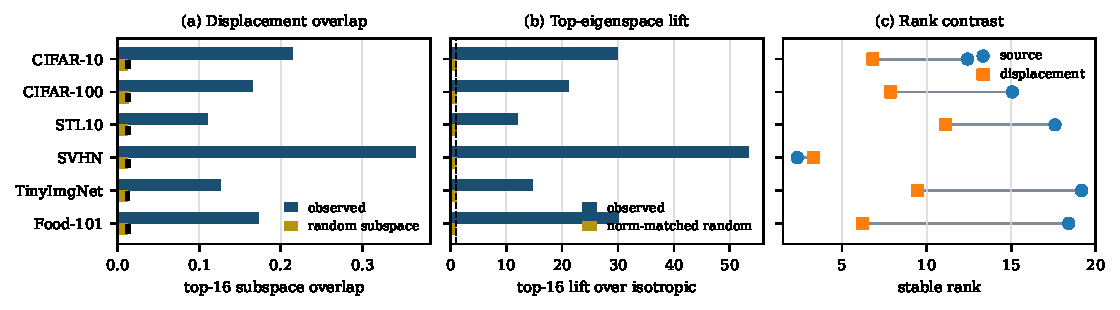
\includegraphics[width=0.98\linewidth]{figures/ijepa_feature_anchor.pdf}
  \caption{Frozen I-JEPA features show covariance-relative view-transfer structure across six standard vision benchmarks. Thirty balanced images per benchmark are encoded with the official frozen I-JEPA ViT-H/16 model under horizontal flips. Panels compare source/displacement top-16 overlap against a random-subspace null, displacement top-eigenspace lift against a norm-matched random-direction control, and source versus displacement stable rank.}
  \label{fig:ijepa-view-transfer}
\end{figure}

This frozen I-JEPA experiment evaluates covariance-relative view transfer across six standard vision benchmarks. The top-16 source/displacement overlap ranges from $0.11062$ to $0.36572$, compared with random-subspace means near $0.0124$. The corresponding top-16 energy lifts range from $12.01$ to $53.33$, while norm-matched random directions remain near one. The effect is therefore shared across datasets but not constant in magnitude, consistent with a covariance-relative rather than spectrum-only description of the view displacement.

An operator-fit stress test complements this positive view-transfer result.
Across five held-out fits (CIFAR-10 with ranks 8 and 16; scikit-learn-digits
with ranks 8, 16, and 32), held-out $R^2$ ranges from $0.97141$ to $0.99840$,
while the fitted commutator stays below the spectrum-preserving random-basis
null mean in every fit (differences from $-0.00417$ to $-0.09323$). View
predictability and covariance-relative operator identification therefore
separate as estimands even within frozen JEPA features.

\subsection{Held-out Action-Conditioned World Models}
\label{sec:temporal-world-models}

Full-rank commutators reveal strong regime dependence but do not by themselves establish out-of-sample temporal correspondence. On PushT, both JEPA-WM and DINO-WM move from below their spectrum-preserving references at short horizons to above them at $h=4$; on PointMaze, both models remain above the reference across $h=1,2,4$. We therefore fit rank-16 ridge operators on training folds and evaluate held-out episodes. Paired $R^2$ exceeds pair-shuffled $R^2$ at every PointMaze horizon: $0.082/0.183/0.025$ versus $-0.092/-0.094/-0.081$ for JEPA-WM, and $0.935/0.808/0.554$ versus $-0.093/-0.083/-0.065$ for DINO-WM. Prediction error, commutator magnitude, and held-out temporal correspondence are thus distinct properties of the learned transition.

Action-order interventions expose where this correspondence uses the supplied future actions. Deranging five-step action blocks within each episode increases PushT prediction error for JEPA-WM at all horizons and for DINO-WM once a deranged future block enters the rollout. DINO-WM PointMaze remains sensitive at horizons 2 and 4, whereas JEPA-WM PointMaze does not deteriorate under the same intervention. Action-order sensitivity is therefore a property of a particular checkpoint, environment, and horizon, rather than an automatic consequence of a nonzero commutator.

The held-out correspondence is stable to the reconstructed PointMaze membership. Across three splitter seeds and a disjoint tail holdout, the paired-minus-shuffled $R^2$ gap remains positive for both models at every horizon. At $h=8$, however, the JEPA-WM PointMaze paired score is $-0.040$ versus $-0.044$ after shuffling, leaving no clear positive out-of-sample signal. The temporal evidence therefore supports a scoped measurement conclusion: alignment and correspondence are measurable beyond one split, but their strength and action dependence vary with the estimator and rollout regime.

We also tested whether the diagnostic can guide selection among
spectrum-preserving linear probes derived from these frozen checkpoints. A
validation one-step-error constraint followed by a train-only alignment
tie-break reduced pooled horizon-4 transfer regret relative to a random
spectrum-only tie-break for both 17- and 65-candidate families. The effect is
not universal: source-stratified results show that it is concentrated in
JEPA-WM/PointMaze, while PushT and DINO-WM/PointMaze usually have degenerate
feasible candidate sets. Alignment-only selection without the error constraint
is unstable. Thus the learned-checkpoint experiment supports a conditional
selection utility for a frozen linear probe family, not a general learned-model
selection rule or a training objective; the complete stratification appears in
the supplement.

\FloatBarrier
\section{Discussion and Limitations}

The central consequence is a conditional operator-pair protocol. A predictor spectrum describes amplification or suppression in the predictor's own eigenbasis, whereas a latent covariance spectrum describes variation in the representation. The metric-aware commutator, principal angles, spectral-projector overlaps, and non-normality quantify distinct relations between these geometries. Eigenvalue-only reporting can be sufficient only after an additional condition is established, such as simultaneous diagonalization in a declared metric or a readout-specific bound based on a measured alignment, Schur/resolvent term, and (for nonlinear dynamics) local-Jacobian remainder. A small commutator by itself is not such a certificate, and none of these quantities is representation-intrinsic without the declared metric.

This perspective is \emph{complementary to equivariant JEPA} designs such as seq-JEPA \citep{ghaemi2025seqjepa}. Such models use known relative transformations and sequence architecture to induce separate equivariant and invariant representations. Our diagnostic is \emph{group-unspecified}: it neither assumes nor tests a particular group representation. An equivariance law can constrain how a transformation acts without, by itself, making the predictor spectrum sufficient to characterize its relation to the latent covariance. The two analyses therefore answer different questions and can be used together: equivariance constrains transformation structure, while metric-aware commutator, Schur, and projector measurements assess whether the predictor spectrum is sufficient to describe transfer in the learned latent geometry.

The learned-representation measurements instantiate this principle at three scales. Frozen LeWM PushT latents exhibit top-band and transition-overlap structure relative to randomized controls. Frozen I-JEPA features exhibit covariance-relative view-displacement structure across six benchmarks, while held-out operator fits separate view predictability from stable operator identification. Released JEPA-WM and DINO-WM checkpoints further separate same-sample commutator scale, held-out temporal correspondence, and sensitivity to action order.

These results establish the portability of the estimands, rather than a universal ordering for learned models. The learned operators are local linear summaries of a particular checkpoint, split, context window, and horizon; the metric-aware commutator is a diagnostic of covariance-relative mismatch, not by itself a causal measure of planning or control quality. For non-normal predictors, Schur-subspace geometry, the resolvent bound, and the non-normality index in Eq.~\eqref{eq:nonnormality-index} are required alongside the commutator; for nonlinear predictors, the local-Jacobian remainder is an additional term rather than a footnote. Establishing a causal link requires matched interventions or downstream evaluations that vary alignment while controlling prediction accuracy. Within this scope, the operator-pair formulation converts a spectrum-only explanation into a testable hypothesis with an explicit metric, estimand, finite-horizon certificate, and null comparison.

The PushT experiments provide a bounded functional consequence of this
distinction. A learned contact adapter and a continuous goal-conditioned
macro-action ranker improve the ordering and final pose quality of available
candidates under a privileged simulator-state protocol. Across the matched
high-coverage evaluation, continuous ranking reduces final block-XY error by
$13.47$ pixels (95\% CI $[-23.48,-4.93]$) and final angle error by
$0.079$ radians (CI $[-0.153,-0.017]$), while the strict-success change is
compatible with zero. This separates continuous pose improvement from
thresholded task completion: local action structure is detectable, but that
detectability is not by itself decision sufficiency.

The candidate interventions identify the next boundary. Enlarging the
absolute-action fan changes oracle coverage only weakly, and matching the
training distribution to the dense fan improves offline selected feasibility
without producing a stable closed-loop success gain. The equal-budget
geometry-conditioned intervention is more diagnostic: oracle availability
increases by $+0.148$ (95\% CI $[+0.086,+0.219]$), whereas frozen-ranker
selected feasibility changes by $-0.023$ (CI $[-0.086,+0.039]$) and selected
contact decreases by $-0.172$ (CI $[-0.242,-0.109]$). Thus candidate
availability, learned ranking, and contact-safe selection are distinct
quantities; reporting only the best available action or the offline ranker
score would hide the failure mode.

A second boundary is physical observability. Cross-fitted readouts can predict
source-defined encoded-latent bands beyond action summaries and remain
informative across longer horizons, but the same coordinates do not improve a
physical-displacement target. The external and intervention audits therefore
support a scoped statement about frozen latent predictability, not a causal
action effect, physical counterfactual, or online planning capability. This
negative transfer is central to the paper's interpretation: a covariance--
predictor alignment statistic can identify structure in a representation
without certifying that the representation is sufficient for a downstream
physical decision.

The privileged planning-interface control clarifies why the final closure gap
should not be attributed to a single estimator. Receding block-pose planning
with contact reacquisition and a separate return objective achieves $16/16$
matched privileged simulator-state closures versus $0/16$ for the coupled
joint-endpoint objective. This result is a control-interface repair, not a
visual LeWM planning result. In combination with the candidate intervention,
it shows that objective decomposition can remove one failure mode while the
learned adapter still lacks stable multi-step pose closure.

Taken together, the PushT evidence is a boundary study for the measurement
principle rather than a claim that LeWM is already a universal world model.
The evidence supports the following operational consequence: a latent spectral
analysis should report (i) covariance--predictor eigenspace alignment, (ii)
candidate availability and selected-action quality when decisions are
evaluated, and (iii) induced-state closure when a controller is claimed. The
complete protocols, seed-level results, action-order controls, and negative
physical-readout audits are provided in the supplement. These measurements
remain complementary to equivariant JEPA architectures: equivariance can
constrain how transformations act, whereas the present group-unspecified
diagnostic tests whether an operator spectrum is sufficient to describe its
relation to latent covariance.

The principal limitations are scope and identification. The exact commutator
identity is proved for the stated finite-dimensional single-plane construction;
learned checkpoint operators are local, estimator-dependent summaries.
PushT experiments use privileged simulator state and offline successor labels,
not visual observations at runtime. The current evidence therefore does not
establish visual online planning, physical causal latent dynamics, universal
world modeling, or a general task-success improvement. The value of the
negative results is that they delimit the conditions under which a positive
spectral or local-readout signal can be interpreted as decision-relevant.
\section{Conclusion}

Predictor eigenvalues do not identify latent transfer without the eigenspaces on which they act. The finite-dimensional isospectral family proves this failure exactly, controlled perturbations isolate covariance--predictor alignment as the mechanism, and measurements in LeWM, I-JEPA, JEPA-WM, and DINO-WM show how the resulting estimands behave in learned representations. The practical rule is simple: a spectral-transfer analysis should state a shared-eigenbasis assumption or report an alignment statistic alongside the spectrum. This operator-pair view turns spectral description into a falsifiable account of which latent directions a learned transition actually transports.

\section*{Supplementary Material}

The supplement includes the complete derivation and rotation sweep, spectrum-preserving nulls, factor-isolating and robustness analyses, frozen PushT and I-JEPA measurements, alignment-intervention boundaries, and full protocols for the held-out JEPA-WM and DINO-WM temporal evaluations.

\section*{Reproducibility Statement}

The theory experiments are deterministic analytical simulations generated from the accompanying source code and stored numerical outputs. Frozen PushT measurements use stored offline latent records; I-JEPA measurements use the official frozen ViT-H/16 checkpoint and deterministic image-view pairs; temporal experiments use released JEPA-WM and DINO-WM checkpoints with the splits and preprocessing specified in the supplement. The accompanying package includes manuscript sources, figures, bibliography and style files, experiment scripts, numerical results, and compiled PDFs.

\bibliographystyle{iclr2027_conference}
\bibliography{references}

\end{document}
